\documentclass[a4paper]{report}

\usepackage{hyperref}
\hypersetup{
    colorlinks,
    citecolor=black,
    filecolor=black,
    linkcolor=black,
    urlcolor=black
}

\usepackage{url}
\usepackage{amsmath}
\usepackage{verbatim}   		% Useful for program listings
\usepackage[T1]{fontenc}       	% For Swedish characters ÅÄÖ etc.
\usepackage[utf8]{inputenc}
% \usepackage[swedish]{babel} % For Swedish hyphenation
\usepackage{fancyvrb}           	% For lists with tabulators
\fvset{tabsize=4}              	 	% Tabulator size
\fvset{fontsize=\small}         	% List font size
\usepackage[nottoc,numbib]{tocbibind}
\usepackage{graphicx}		% Imports the graphicx package, useful for images
% \usepackage{}
% \makeatletter\@addtoreset{chapter}{part}\makeatother% % Makes chapter numbering reset after each part
\usepackage[scaled=0.8]{beramono} % changes font of all ttfamily text, like code listings and links. Default makes "+=" look ugly in code listing
\usepackage{listingsutf8}
\lstset{
  basicstyle=\scriptsize\ttfamily,
  language=C,
  extendedchars=true,
  inputencoding=utf8,
  commentstyle=\color{black},
  gobble=12
}

\title{Dragonfly Quadrotor UAV \\ Flight Control Board}
\author{Nina Khayyami \\ Adam Steineck \\ Daniel Stenberg }

\date{\today}         			% Sets date on first page

\begin{document}                	% Start of document

\maketitle                      		% Prints the title defined above with \title, \author and \date
\begin{verbatim}Copyright (C)  2016 ÅF AB.
    Permission is granted to copy, distribute and/or modify this document
    under the terms of the GNU Free Documentation License, Version 1.3
    or any later version published by the Free Software Foundation;
    with no Invariant Sections, no Front-Cover Texts, and no Back-Cover Texts.
    A copy of the license is included in the section entitled "GNU
    Free Documentation License".
\end{verbatim}
\newpage
\tableofcontents				% Insert table of contents

\newpage

\chapter{List of Abbreviations}

\chapter{Introduction}

The \emph{Dragonfly} project is an internal competence enhancement project for ÅF employees. The goal is to combine technology, competence and experience from various engineering fields in order to construct a highly advanced quadrotor UAV system. The focus of the Flight Control Board development deals with low-level maneuvering of the aircraft, calculating motor command based on a feedback control system. Some of the major technologies deployed to attain this are control theory, electronics and software development.

An early CAD rendeded image of the Dragonfly quadrotor concept can be viewed in Figure \ref{fig:quadrendered1}.

\begin{figure}[h]
    \centering
    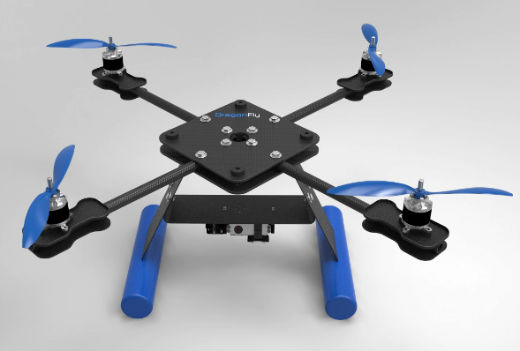
\includegraphics[scale=0.4]{images/quad_concept1_rendered.jpg}
    \caption{Rendered image of one of the first quadrotor designs concepts}
    \label{fig:quadrendered1}
\end{figure}

%
% THEORY PART STARTS HERE!
%
\part{Theory}

\chapter{Introduction}
This part concerns the physical, mathematical and control system theory essential to understand the quadrotor system sufficiently to control its flight. The flight theory presents a rigid-body dynamical model of the quadrotor flight as well as representation of coordinate systems suitable to present aircraft states such as position, attitude and velocity. Aerodynamic effects on this system is also presented and discussed. For the control part, the problem of controlling the aircraft is split in to two distinct parts - estimating the current states and controlling the system to achieve desired states.

\chapter{System Description}

	\section{Coordinate System Representation}
World-frame and body-frame coordinate systems. Euler angles and rotation matrices. Transformations between coordinate frames.

	\section{Flight Dynamics}

	\section{BLDC Motor Theory}
	\label{sec:BLDCMotorTheory}
Brushless DC electric motor (BLDC motors, BL motors) also known as electronically commutated motors (ECMs, EC motors) are synchronous motors that are powered by a DC electric source via an integrated inverter/switching power supply, which produces an AC electric signal to drive the motor. In this context, AC, alternating current, does not imply a sinusoidal waveform, but rather a bi-directional current with no restriction on waveform. Additional sensors and electronics control the inverter output amplitude and waveform (and therefore percent of DC bus usage/efficiency) and frequency (i.e. rotor speed).

Electrical motors are based on interaction between two magnetic fields, one produced by a permanent magnet and one by current flowing in the motor windings. The fields produce a torque which drives the rotor. During rotation, the current in the winding is commutated (reversed) to obtain a continuous torque.

The BLM motors used for this project have an “outrunner” architecture, which means that the permamagnet rotor lies outside the winding stator. The windings are separated into several coils energized cyclically (AC current) by an electronic speed controller (ESC) to achieve rotor rotation.

	\section{Radio Control Theory}

	\section{Sensor Theory}

		\subsection{Microelectromechanical Systems (MEMS) Sensors}

		\subsection{Gyroscope}

		\subsection{Accelerometer}

		\subsection{Magnetometer}

\chapter{State Estimation Theory}
\label{chap:state-estimation-theory}
	\section{Attitude Estimation}
Dragonfly uses a Kalman filter to estimate the roll, pitch and yaw angles. The state vector for the attitude is the attitude angle and the angular rate bias. The latter is due to gyroscope having a drift in its measured angular velocity, that is, taking a number of samples and averaging the value and using this as an offset. in the below equations, steps 1-2 are the prediction step of the Kalman filter and 3-7 the correction step. The estimation step for roll, pitch and yaw is run when the gyroscope values  are updated, these are angular velocities in rad/s. The correction step for roll and pitch is run when the accelerometer values are available. The correction step for yaw is run when magnetometer values are available.
	\subsection{Two value state vector version}
	The state vector is the angle $\theta$  and angle rate bias $\dot{\theta}_b$. In this version the gyroscope is used as the input $u$.

		Step 1: Predict the estimated states $\hat{x}_{k|k-1}$
		\begin{equation}
		\label{eq:state-equation-2v}
		\hat{x}_{k|k-1}=A\hat{x}_{k-1|k-1}+Bu_{k}
		\end{equation}

		\begin{equation}
		\label{eq:state-equation-detailed}
		\left[
      		\begin{array}{c}
      		\hat{\theta}\\
		\hat{\dot{\theta}}_{b}
      		\end{array} \right]_{k|k-1}
		=
		\left[
		\begin{array}{c c}
		1 & - \Delta T\\
		0 & 1
		\end{array} \right]
		\left[
		\begin{array}{c}
		\hat{\theta}\\
		\hat{\dot{\theta}}_{b}
		\end{array} \right]_{k-1|k-1}
		+
		\left[
		\begin{array}{c}
		\Delta T\\
		0
		\end{array} \right]
		\dot{\theta}_{gyro, k}\\
		\end{equation}
		\begin{equation}
		z_{k}=
		\left[
		\begin{array}{c c}
		1 & 0
		\end{array} \right]
		\left[
		\begin{array}{c}
		\theta\\
		\dot{\theta}_{b}
		\end{array} \right]_{k|k-1}
		\end{equation}
    In pseudo code:
    \begin{lstlisting}[frame=single]
		predictAngle = angle + dt*gyroRate - dt*bias;
		//gyroRate is the rate from the gyroscope
		predictBias = bias;
		\end{lstlisting}

		Step 2: Predict the error covariance matrix $P_{k|k-1}$,
		\begin{equation}
		\label{eq:error-covariance-prediction}
		P_{k|k-1}=AP_{k-1|k-1}A^{T}+Q
		\end{equation}

		where $Q$ is the process noise covariance matrix, in this application, $q_{00}$ this is the measured gyroscope error variance.

		\begin{equation}
		\label{eq:error-covariance-prediction-detailed}
		\left[
		\begin{array}{c c}
		P_{11}	&	P_{12}\\
		P_{21}	&	P_{22}
		\end{array} \right]_{k|k-1}
		=
		\left[
		\begin{array}{c c}
		1 & - \Delta T\\
		0 & 1
		\end{array} \right]
		\left[
		\begin{array}{c c}
		P_{11}	&	P_{12}\\
		P_{21}	&	P_{22}
		\end{array} \right]_{k-1|k-1}
		\left[
		\begin{array}{c c}
		1	&	0\\
		- \Delta T & 1
		\end{array} \right]
		+
		\end{equation}
		\begin{equation}
		+
		\left[
		\begin{array}{c c}
		\sigma(\dot{\theta}_{gyro})\cdot\Delta T^{2}	&	0\\
		0	&	 \sigma(\dot{\theta_{b}})
		\end{array} \right]
		\end{equation}
    In pseudo code:
		\begin{lstlisting}[frame=single]
		P11 += dt*(dt*P22 - P12 - P21 + Q1);
		P12 -= dt*P22;
		P21 -= dt*P22;
		P22 += dt*Q2;
		\end{lstlisting}
		Step 3: Now calculate the difference $\tilde{y}_{k}$ between the predicted state $\hat{x}_{k|k-1}$ and the measurement $z_{k}$
		\begin{equation}
		z_{k}=H\hat{x}_{k|k-1}
		\end{equation}
		\begin{equation}
		\tilde{y}_{k}=z_{k}-H\hat{x}_{k|k-1}
		\end{equation}
		The extraction matrix $H$ matrix defines what sensor readings we would get under the conditions that our $\hat{x}$ was perfectly estimated and our sensors delivered perfect values.\footnote{See  \url{https://www.udacity.com/wiki/cs373/kalman-filter-matrices}}

		\begin{equation}
		\tilde{y}_{k}=z_{k}-\left[
		\begin{array}{c c}
		1	&	0
		\end{array} \right]
		\left[
		\begin{array}{c}
		\theta \\
		\dot{\theta}_{b}
		\end{array} \right]_{k|k-1}
		\end{equation}
    In pseudo code:
		\begin{lstlisting}[frame=single]
		y = sensorAngle - predictAngle;
		//sensorAngle is the angle computed from sensor values
		\end{lstlisting}
		Step 4: Calculate the innovation covariance matrix $S_{k}$
		\begin{equation}
		\label{eq:innovation-covariance-matrix}
		S_{k}=HP_{k|k-1}H^{T}+R
		\end{equation}

		where $R$ is the measurement noise covariance matrix, in this application this the measured variance of the $\theta$ angles calculated from the accelerometer.

		\begin{equation}
		S_{k}=
		\left[
		\begin{array}{c c}
		1	&	0
		\end{array} \right]
		\left[
		\begin{array}{c c}
		P_{11}	&	P_{12}\\
		P_{21}	&	P_{22}
		\end{array} \right]_{k|k-1}
		\left[
		\begin{array}{c}
		1\\
		0
		\end{array} \right]
		+ \sigma(\theta_{acc})
		\end{equation}

		where
		\begin{equation*}
		\theta_{acc}=\arctan{\left(\frac{a_{y}}{a_{z}}\right)}
		 \end{equation*}
    In pseudo code:
		\begin{lstlisting}[frame=single]
		S = P11 + R;
		\end{lstlisting}
		Step 5: Calculate the Kalman gain $K_{k}$
		\begin{equation}
		\label{eq:kalman-gain}
		K_{k}=P_{k|k-1}H^{T}S^{-1}_{k}
		\end{equation}

		\begin{equation}
		\left[
		\begin{array}{c}
		K_{1}\\
		K_{2}
		\end{array} \right]_{k}
		=
		\left[
		\begin{array}{c c}
		P_{11}	&	P_{12}\\
		P_{21}	&	P_{22}
		\end{array}  \right]_{k|k-1}
		\left[
		\begin{array}{c}
		1\\
		0
		\end{array} \right]
		S^{-1}_{k}
		\end{equation}
    In pseudo code:
		\begin{lstlisting}[frame=single]
		K1 = P11 / S;
		K2 = P21 / S;
		\end{lstlisting}
		Step 6: Update the state prediction $\hat{x}_{k|k-1}$ to  $\hat{x}_{k|k}$
		\begin{equation}
		\label{eq:correct-state-estimation}
		\hat{x}_{k|k}=\hat{x}_{k|k-1}+K_{k}\tilde{y}_{k}
		\end{equation}

		\begin{equation}
		\left[
		\begin{array}{c}
		\theta\\
		\dot{\theta}_{b}
		\end{array} \right]_{k|k}
		=
		\left[
		\begin{array}{c}
		\theta\\
		\dot{\theta}_{b}
		\end{array} \right]_{k|k-1}
		+
		\left[
		\begin{array}{c}
		K_{1}\\
		K_{2}
		\end{array} \right]_{k}
		\tilde{y}_{k}
		\end{equation}
    In pseudo code:
		\begin{lstlisting}[frame=single]
		correctAngle = predictAngle + K[0]*y;
		correctBias = predictBias + K[1]*y;
		\end{lstlisting}
		Step 7: Update the error covariance matrix prediction $P_{k|k-1}$ to $P_{k|k}$
		\begin{equation}
		\label{correct-error-covariance}
		P_{k|k}=(I-K_{k}H)P_{k|k-1}
		\end{equation}

		\begin{equation}
		\left[
		\begin{array}{c c}
		P_{11}	&	P_{12}\\
		P_{21}	&	P_{22}
		\end{array} \right]_{k|k}
		=
		\left(
		\left[
		\begin{array}{c c}
		1	&	0\\
		0	&	1
		\end{array} \right]
		-
		\left[
		\begin{array}{c}
		K_{1}\\
		K_{2}
		\end{array} \right]_{k}
		\left[
		\begin{array}{c c}
		1	&	0
		\end{array} \right]
		\right)
		\left[
		\begin{array}{c c}
		P_{11}	&	P_{12}\\
		P_{21}	&	P_{22}
		\end{array} \right]_{k|k-1}
		\end{equation}
    In pseudo code:
		\begin{lstlisting}[frame=single]
		float P11_tmp = P11;
		float P12_tmp = P12;

		P11 -= K1*P11_tmp;
		P12 -= K1*P12_tmp;
		P21 -= K2*P11_tmp;
		P22 -= K2*P12_tmp;
		\end{lstlisting}
	\subsection{Attitude estimation using three value state vector}
		In this version {\url{www.linushelgesson.se/2012/04/pitch-and-roll-estimating-kalman-filter-for-stabilizing-quadrocopters}}, the state vector is the angle $\theta$, the angular rate $\dot{\theta}$ and angular rate bias $\dot{\theta}_b$. The matrix $B$ in the state equation \ref{eq:state-equation-2v} is set to zero due to the complexity of accurately modelling the impact of control input $u$ on the state vector but this may be added in future versions.

[TODO: Add information and pseudo-code on how to include B matrix and system input]

[TODO: Needs review and correcting, S matrix seems wrong...]

		Step 1: Predict the estimated states $\hat{x}_{k|k-1}$
		\begin{equation}
		\hat{x}_{k|k-1}=A\hat{x}_{k-1|k-1}
		\end{equation}
		\begin{equation}
		\left[
      		\begin{array}{c}
      		\hat{\theta}\\
		\hat{\dot{\theta}}\\
		\hat{\dot{\theta}}_{b}
      		\end{array} \right]_{k|k-1}
		=
		\left[
		\begin{array}{c c c}
		1 &   \Delta T & - \Delta T\\
		0 & 1 & 0 \\
		0 & 0 & 1 \\
		\end{array} \right]
		\left[
		\begin{array}{c}
		\hat{\theta}\\
		\hat{\dot{\theta}}\\
		\hat{\dot{\theta}}_{b}
		\end{array} \right]_{k-1|k-1}
		\end{equation}
		Selecting a measurement vector $z$ at time $k$,
		\begin{equation*}
		z_k =
		\left[
		\begin{array}{c}
		\theta\\
		\hat{\theta}
		\end{array}
		\right]
		\end{equation*}
		the measurement equation
		\begin{equation}
		z_k = H x_k
		\end{equation}
		\begin{equation}
		\label{eq:measurement-equation-3v}
		z_{k}=
		\left[ \begin{array}{c c c}
		1 & 0 & 0\\
		0 & 1 & 0
		\end{array} \right]
		\left[
      		\begin{array}{c}
      		\theta\\
		\dot{\theta}\\
		\dot{\theta}_{b}
		\end{array} \right]_{k|k-1}
		\end{equation}
		shows the extration matrix $H$.
		\subsubsection{Three value state vector prediction step}
		Equation \ref{eq:error-covariance-prediction} for the three value state vector becomes:
		\begin{equation}
		\label{eq:error-covariance-prediction-3v}
		P_{k|k-1}
		=
		\left[	\begin{array}{c c c}
		1 &   \Delta T & - \Delta T\\
		0 & 1 & 0 \\
		0 & 0 & 1 \\
		\end{array} \right]
		P_{k-1|k-1}
		\left[	\begin{array}{c c c}
		1 &  0 & 0 \\
		\Delta T  & 1 & 0 \\
		-\Delta T  & 0 & 1 \\
		\end{array} \right]
		+ Q
		\end{equation}
		where
		\begin{equation}
		\label{eq:P-3v}
		P =
		\left[
		\begin{array}{c c c}
		P_{11} & P_{12} & P_{13} \\
		P_{21} & P_{22} & P_{23} \\
		P_{31} & P_{32} & P_{33}
		\end{array}\right]
		\end{equation}
		and the constant matrix $Q$ is given by
		\begin{equation}
		\label{eq:Q-3v}
		Q =
		\left[ \begin{array}{c c c}
		Q_{11} & 0 & 0 \\
		0 & Q_{22} & 0 \\
		0 & 0 & Q_{33}
		\end{array} \right]
		\end{equation}
		The matrix $Q$ will initially be selected to give a value of the Kalman gain similtar to those achieved by the two-value state vector version, as the Kalman gain is dependent on the ratio between the measurement noise $R$ and process noise $Q$, but there is no method to directly measure the process noise.
		Solving equations \ref{eq:error-covariance-prediction-3v} and \ref{eq:P-3v} by hand gives the following  pseudo code for predicting the error covariance matrix:
		\begin{lstlisting}[frame=single, label={eq:error-covariance-prediction-3v},caption={Error covariance prediction pseudo code}]
		P11 += P11 + dt * P21 - dt * P31
		       + dt * (P12 + dt * P22 - dt * P32)
		        - dt * (P13 + dt * P23 - dt * P33)
		        + Q11
		P12 += dt * (P22 - P32)
		P13 += dt * (P23 - P33)
		P21 += dt * (P22 - P23)
		P22 += Q22
		P31 += dt * (P32 - P33)
		P33 += Q33
		// P23, P32  not updated
		\end{lstlisting}
		which will drive the update or estimation step of the Kalman filter.
		\subsubsection{Three value state vector correction step}
		Equation \ref{eq:innovation-covariance-matrix} for calculating the error innovation covariance matrix $S_{k}$ becomes the below for the three value state vector variant:
		\begin{equation}
		\label{eq:innovation-covariance-matrix-3v}
		S_{k} =
		\left[ \begin{array}{c c c}
		1 & 0 & 0 \\
		0 & 1 & 0
		\end{array} \right]
		\left[
		\begin{array}{c c c}
		P_{11} & P_{12} & P_{13} \\
		P_{21} & P_{22} & P_{23} \\
		P_{31} & P_{32} & P_{33}
		\end{array}\right]_{k-1|k-1}
		\left[ \begin{array}{c c}
		1 & 0 \\
		0 & 1 \\
		0 & 0
		\end{array} \right]
		+ R
		\end{equation}
		which become the below after matrix multiplications and substituting the diagonal elements of $R$ into the variances for the accelerometer derived angles and gyroscope angular velocity respectively.
		\begin{equation}
		S_{k} =
		\left[ \begin{array}{c c}
		P_{11} & P_{12} \\
		P_{21} & P_{22}
		\end{array} \right]
		+
		\left[ \begin{array}{c c}
		\sigma(\theta_{acc}) & 0 \\
		0 & \sigma(\dot{\theta}_{gyro})
		\end{array} \right]
		\end{equation}
		which is used to derive the Kalman gain according to equation \ref{eq:kalman-gain}, which in the three value state vector becomes an 3 by 2 matrix $K$:
		\begin{equation}
		\label{eq:kalman-gain-3v}
		K_k  =
		\frac{1}{det(S)}
		  \left[ \begin{array}{c c}
		      P_{11}(P_{22} + \sigma(\dot{\theta}_{gyro})) - P_{12}P_{21} & -P_{12}\sigma(\theta_{acc}) \\
          P_{21}\sigma(\dot{\theta}_{gyro})                           & -P_{21}P_{12} + P_{22}(P_{11} + \sigma(\theta_{acc}))\\
          P_{31}(P_{22}+\sigma(\dot{\theta}_{gyro})) - P_{32}P_{21}   & -P_{31}P_{12}+P_{32}(P_{11}+\sigma(\theta_{acc}))
		    \end{array} \right]
		\end{equation}
		where $det(S)$ is the determinant of matrix $S$ which results from the $S^{-1}$ term of equation \ref{eq:kalman-gain} and its expression is:
		\begin{equation}
		det(S) = P_{22}(P_{11} + \sigma(\theta_{acc}) - P_{12})
		\end{equation}



		See equation \ref{eq:correct-state-estimation} for the expression to correct the state estimation. Its term $y_k$ for the difference between the estimated state and the measured angle and angular rate in three value state vector variant then becomes:
		\begin{equation}
		\label{eq:state-meas-difference-3v}
		y_k =
		\left[ \begin{array}{c}
		y_1 \\
		y_2
		\end{array} \right]
		=
		\left[ \begin{array}{c}
		\theta_{acc} - \hat{\theta}_{acc} \\
		\dot{\theta}_{gyro} - \hat{\dot{\theta}}_{gyro}
		\end{array} \right]
		\end{equation}
		The pseudo code for doing equation \ref{eq:correct-state-estimation} in the three value state vector version follows:
		\begin{lstlisting}[frame=single, caption={Correct state estimate pseudo code}, label={pseudo:correct-state-estimate-3v}]
		y1 = angleMeasured - angleEstimated
		y2 = angleDotMeasured - angleDotEstimated

		 detS = P22 * (P11 + angleVariance - P12)

		K11 = 1 / detS * (P11 * (P22 + angleDotVariance)) - P12 * P21)
		K12 = 1 / detS * -P12 * angleVariance
		K21 = 1 / detS * P21 * angleDotVariance
		K22 = 1 / detS * (-P21 * P12 + P22 * (P11 + angleVariance))
		K31 = 1 / detS * (P31 * (P22 + angleDotVariance) - P32 * P21)
		K32 = 1 / detS * (-P31 * P12 + P32 * (P11 + angleVariance))

		angleEstimated		+=  K11 * y1 + K12 * y2
		angleDotEstimated	+=  K21 * y1 + K22 * y2
		angleDotBiasEstimated	+=  K31 * y1 + K32 * y2
		\end{lstlisting}
		The error covariance correction is given by equation \ref{correct-error-covariance}. Using extraction matrix $H$ from equation \ref{eq:measurement-equation-3v} and  the Kalman gain $K_{k}$ from equation \ref{eq:kalman-gain-3v} the expression for the corrected $P$ becomes:
		\begin{equation}
		P_{k|k} =
      		\left[ \begin{array}{c c c}
	          1 - K_{11} & - K_{12} & 0 \\
	          -K_{21} & 1 - K_{22} & 0 \\
	          -K_{31} & -K_{32} & 1
		\end{array} \right]
		\left[ \begin{array}{c c c}
		P_{11} & P_{12} & P_{13} \\
		P_{21} & P_{22} & P_{23} \\
		P_{31} & P_{32} & P_{33}
		\end{array}\right]_{k-1|k-1}
		\end{equation}
		Re-using the Kalman gain from pseudo code \ref{pseudo:correct-error-covariance-3v}, the pseudo code for updating the error covariance becomes:
		\begin{lstlisting}[frame=single, caption={Correct state estimate pseudo code}, label={pseudo:correct-error-covariance-3v}]
		// note that that values P1[1-3] and P2[1-3] must be copied to temporary values for
		// RHS expressions to yield the correct values
		P11 -= K11 * P11 + K12 * P21
		P12 -= K11 * P12 + K12 * P22
		P13 -= K11 * P13 + K12 * P23

		P21 -= K21 * P11 + K22 * P21
		P22 -= K21 * P12 + K22 * P22
		P23 -= K21 * P13 + K22 * P23

		P31 -= K31 * P11 + K32 * P21
		P32 -= K31 * P12 + K32 * P22
		P33 -= K31 * P13 + K32 * P23
		\end{lstlisting}
	\section{Velocity Estimation}
	Kalman filters are used to estimate the angles, $\theta_{k}$, and in order to find the angular velocity, $\dot{\theta}_{k}$, we can calculate the derivative of the angle. Equation \ref{eq:kalman-gain} for the three value state vector becomes:
	\begin{equation}
	\label{thetaDot}
	\dot{\theta}_{k}=\frac{\theta_{k}-\theta_{k-1}}{\Delta T}
	\end{equation}


\chapter{Flight Control Theory}

	\section{Control Design Overview}

Figure \ref{fig:controloverview} shows an overview of the control problem.

\begin{figure}[h]
    \centering
    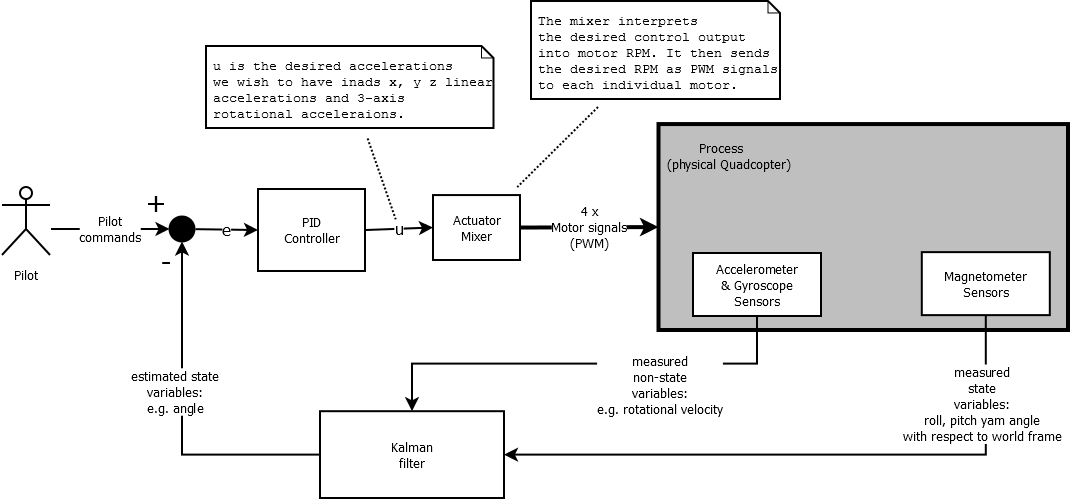
\includegraphics[scale=0.3]{images/ControlDiagram.png}
    \caption{Control overview diagram}
    \label{fig:controloverview}
\end{figure}

	\section{PID Control}

		\subsection{The algorithm}
The PID control strategy is one of the most commonly used control algorithms. It consists of three parts that each contribute to the control signal; Proportional (P), Integral (I) and Derivative (D). The equation for the PID algorithms is presented in (\ref{PID_classic}), where $u(t)$ is the control signal and $e(t) = y_{ref}(t) - y(t)$ is the control error. This is the classical representation without any modifications. When used in practice, some alterations are typically made to address some practical issues and increase performance in a real-world environment. For one, it needs to be discretized so that a digital computer may generate control signals, but there are numerous other modifications to consider.

\begin{equation}
u(t) = K \bigg( e(t) + \dfrac{1}{T_i} \int_{0}^{\infty}  e(t) dt + T_d \dfrac{d}{dt} e(t) \bigg)
\label{PID_classic}
\end{equation}

When tuning the algorithm (\ref{PID_classic}), a set of parameters $K$, $T_i$, $T_d$ are selected by, for example, pole placement, step response analysis or frequency diagram design.

	\subsection{Practical modifications}
To ensure performance in a real-world environment, a number of modifications are typically made to address the following issues:

\begin{itemize}
\item High-frequency noise
\item Integrator wind-up due to saturation
\item Transfer between control parameters and modes
\end{itemize}

Along with this, a few other parameters are introduced enable more possibilities to achieve desired performance.

	\subsection{Discretization}
To run the algorithms on a digital system, the equation needs to be discretized. This is often achieved using a finite-step approximation such as backward and forward difference or Tustin approximation.

	\section{Attitude Control}

	\section{Velocity Control}

\chapter{Sensor Calibration Algorithms}

	\section{Gauss-Newton Optimization}

	\section{Magnetometer calibration}

	\section{Accelerometer calibration}

%
% IMPLEMENTATION PART STARTS HERE!
%
\part{Implementation}

\chapter{Introduction}
In this part, the implementation of the flight control system is presented and discussed. It concerns documentation of both electronic and software design choices. The heart of the flight control system is the \emph{Flight Control Board} (FCB) program, running on an STM32F303VC microcontroller attached to an STM32F3Discovery board featuring on-board sensors, debug interface and more. The program is mainly written in C code and executes code to, among other things, control and actuate the motors, read from the sensors and an RC receiver and estimate the flight states.

\chapter{Hardware}

	\section{Flight Control Board - STM32F3Discovery}
The STM32F3Discovery is an evaluation board provided by STMicroelectronics. It features an STM32F303VCT6 microprocessor based on the ARM Cortex-M4 core. For evaluation purposes, the board has been fitted with accelerometer, magnetometer and gyroscope sensors, an on-board ST-Link/V2 debugger/programmer, various LED:s, extension headers for all I/O pins and more.

\begin{itemize}
  \item CPU speed: $72$ MHz
  \item ROM: $256$ kB Flash
  \item RAM: $48$ kB ($40$ kB SRAM, $8$ kB CCM)
  \item I/O pins: LQFP100 pin package with pins attached to extension header
  \item On-board ST-LINK/V2 programming and debugging device
  \item Power supply: From USB bus or from an external $3$ $V$ or $5$ $V$ supply voltage
  \item L3GD20 MEMS gyroscope
  \item LSM303DLHC MEMS accelerometer and magnetometer
  \item 10 LEDs
  \item Two pushbuttons
  \item USB USER Mini-B connector
\end{itemize}

Figure \ref{fig:stm32f3busmatrix} shows the microcontroller internal bus matrix, connecting the core to the MCU peripherals.

\begin{figure}[h]
    \centering
    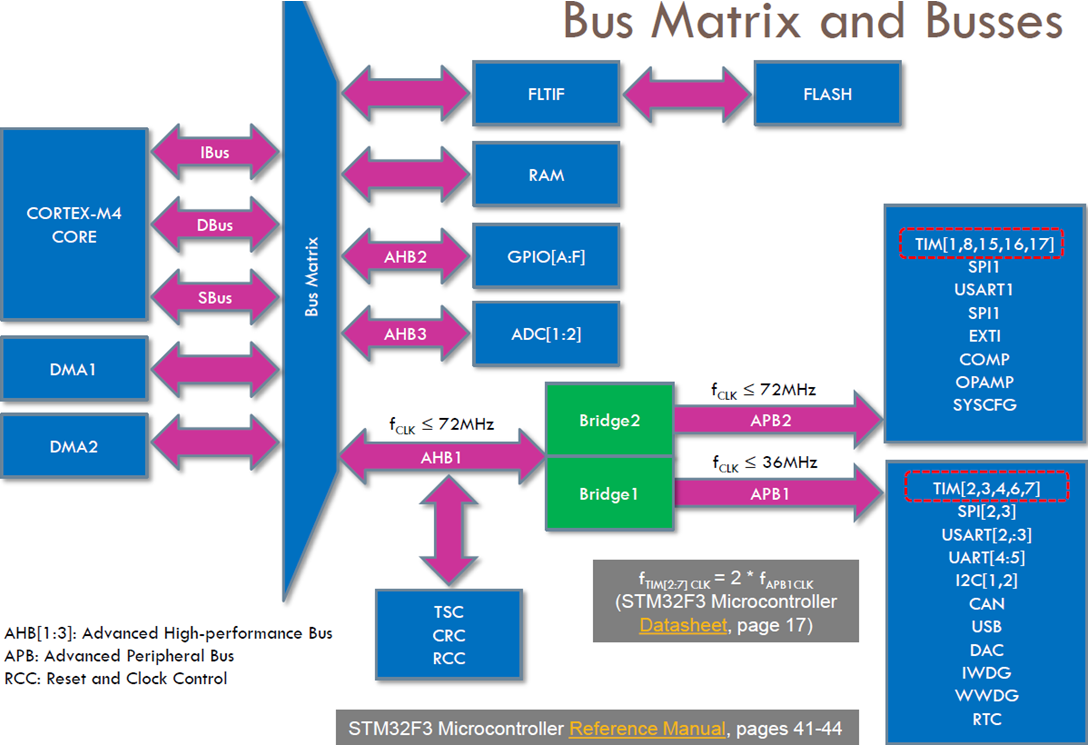
\includegraphics[scale=0.4]{images/stm32_busmatrix.png}
    \caption{STM32F3 bux matrix}
    \label{fig:stm32f3busmatrix}
\end{figure}

	\section{T-Motor U3 BLDC Motors}
The motors of choice for the Dragonfly are of the type \emph{T-motor U3}, which are sensorless (no built-in Hall sensor) brushless motors, designed to deliver high performance and reliability. According to the manufacturer, they are highly resistant to dirt and water. There are several benefits of using brushless motors instead of traditional DC motors, including longer life-time (due to no brushes that become worn out), less noisy operation and more efficient cooling.

The T-motor U3 motors have 12 stator coils and 14 rotor magnets. The motor theory was earlier presented in Section \ref{sec:BLDCMotorTheory}.

\begin{itemize}
  \item Motor velocity constant: $700$ $rpm/V$
  \item Stator-pole configuration: $12N-14P$
  \item Dimensions: Diameter: $41.80$ $mm$, Height: $30.75$ $mm$
  \item Weight: $97$ $g$
  \item Idle current: $0.5$ $A$
  \item Recommended number of battery cells (LiPo): $3-4S$
  \item Max continuous current ($180$ $s$): $25$ $A$
  \item Max continuous power ($180$ $s$): $400$ $W$
  \item Max current efficiency: ($4-10$ $A$) $>82$ \%
  \item Internal resistance: $50$ $m\Omega$
\end{itemize}

\begin{figure}
    \centering
    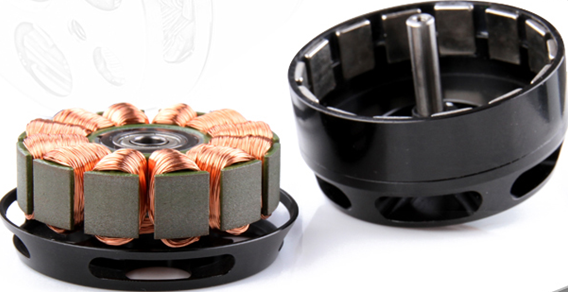
\includegraphics[scale=0.6]{images/tmotoru3open.png}
    \caption{T-Motor U3 BLDC motors}
    \label{fig:tmotoru3open}
\end{figure}

The motor and propeller manufacturer, T-motors, provides some information on the actuation characteristics in Table \ref{table:motorManufacturerData}. The values were obtained with an operating temperature of $43^{\circ}$ $C$ with 11x3.7 inch T-motors carbon fibre propellers attached to the motor shaft.

\begin{table}
\begin{tabular}{ |c|c|c|c|c|c| }
\hline
\textbf{Throttle} & \textbf{Current} & \textbf{Power} & \textbf{Thrust} & \textbf{Speed} & \textbf{Efficiency} \\
\textbf{\%} & \textbf{[$A$]} & \textbf{[$W$]} & \textbf{[$g$]} & \textbf{[$rpm$]} & \textbf{[$g/W$]} \\
\hline
$50$ & $3.2$ & $48$ & $460$ & $5300$ & $9.58$ \\
$65$ & $6.0$ & $87$ & $710$ & $6500$ & $8.16$ \\
$75$ & $8.2$ & $120$ & $870$ & $7500$ & $7.25$ \\
$85$ & $11.0$ & $160$ & $1080$ & $8200$ & $6.75$ \\
$100$ & $13.0$ & $193$ & $1230$ & $8700$ & $6.37$ \\
\hline
\end{tabular}
\caption{T-Motor U3 motor with 11x3.7 inch CF propeller data}
\label{table:motorManufacturerData}
\end{table}

	\section{T-Motor ESC30A Electronic Speed Controllers}
Motor speed control is achieved using ESCs, which cyclically shift the coils’ current by applying a three-phase alternating-current. So the motors themselves are really AC motors, although driven by a DC power source (battery).

The battery drain is determined using MOSFET transistors. By feeding an ESC with a pulse-width modulated (PWM) signal, battery power is switched on and off rapidly for periods decided by the PWM duty cycle. Since this is done at a sufficiently high frequency, the supplied current (which is modulated to AC) “seen” by the motors can be approximated to the mean battery drain. So, the higher the duty cycle the more battery drain and the higher larger electromagnetic torque generated in motor.

The ESCs of choice for this project is the \emph{T-Motor ESC30A}, shown in Figure \ref{fig:esc_tmotor}. It takes a PWM input signal up to $400$ $Hz$ to drive the motors. Normally in RC applications, a $1$ $ms$ pulse width indicates $0$ \% throttle, whereas $2$ $ms$ is 100 \% throttle (with $50$ \% being approx. $1.5$ $ms$). The ESCs feature BEC (Battery eliminator circuit), which outputs a low-power $5$ $V$ source useful to power onboard electronics.

\begin{figure}
    \centering
    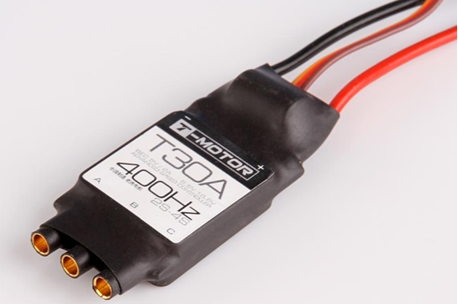
\includegraphics[scale=0.8]{images/esc_tmotor.png}
    \caption{T-Motor ESC30A Electronic Speed Controller}
    \label{fig:esc_tmotor}
\end{figure}

\begin{itemize}
  \item Output: Continuous 30A, Burst 40A up to 10 Secs.
  \item Input: 2-4 cells lithium battery or 5-12 cells NiCd/NIMh battery.
  \item BEC: $2$ $A$ / $5$ $V$ (Linear mode)
  \item Max speed: $35000$ $rpm$ for BLDC motor
\end{itemize}

	\section{RC Receiver and Transmitter}

The Spektrum AR610 receiver, shown in Figure \ref{fig:ar610}, employs full-range $2.4$ GHz DSMX modulated radio communication. It is capable of reading and outputting up to 6 channels of controller information. The output from each channel consists of a PWM signal with a period of $22$ $ms$ (approx. $45.45$ Hz) with a pulse width between (approx.) $1$ and $2$ ms, depending on controller action. There is also an additional receiver output, used for binding the controller with the receiver. The channels are labeled as follows:

\begin{itemize}
  \item BND/DAT (Bind) - Used only to bind the controller to the receiver with the bind plug (see image). More on this can be found in the controller and/or receiver manuals.
  \item THRO (Throttle) – Typically used to control the altitude actuation.
  \item AILE (Aileron) – Typically used to control the roll actuation.
  \item ELEV (Elevator) – Typically used to control the pitch actuation.
  \item RUDD (Rudder) – Typically used to control the yaw actuation.
  \item GEAR – Open to interpretation
  \item AUX (Auxiliary) - Open to interpretation.
\end{itemize}

\begin{figure}
    \centering
    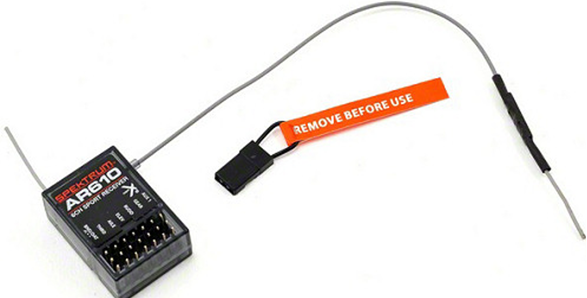
\includegraphics[scale=0.8]{images/ar610.png}
    \caption{Spektrum AR610 receiver}
    \label{fig:ar610}
\end{figure}

The RC transmitter of choice is the Spektrum DX6i, which is a 6-channel transmitter using $2.4$ GHz Spektrum DSMX modulation. In Figure \ref{fig:dx6i_map}, the transmitter's stick and switch mapping and labeling is shown.

\begin{figure}
    \centering
    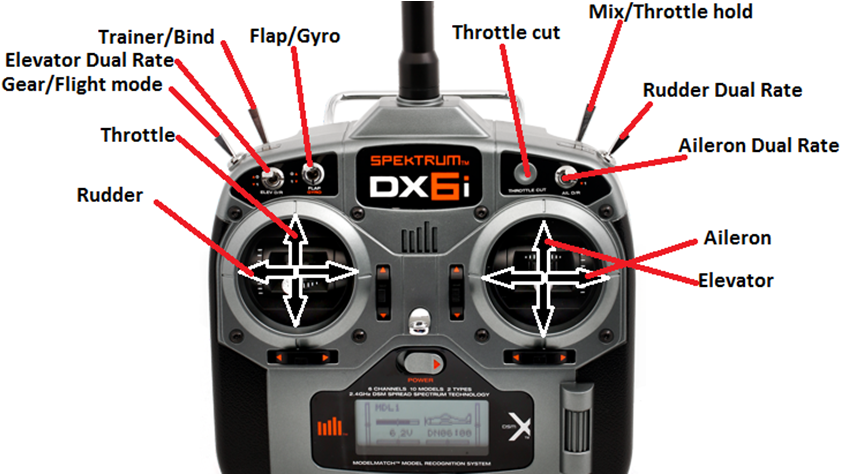
\includegraphics[scale=0.6]{images/dx6i_map.png}
    \caption{Spektrum DX6i RC transmitter labels}
    \label{fig:dx6i_map}
\end{figure}

MCU Timer Input Compare registers are configured and used to read input PWM signals, typically from the RC receiver. They are connected to timer channels to generate interrupts on up and down flanks of PWM pulses (the polarity is reversed after reading each flank).

	\section{Battery}

The battery used is of Lithium polymer type, containing Lithium ions to drive current from the positive to the negative electrode through a closed circuit.

\begin{itemize}
  \item Capacity: $8000$ $mAh$
  \item Voltage: $14.8$ $V$
\end{itemize}

	\section{Sensors}

L3DG20 Gyroscope over SPI. LSM303DLHC over I2C. Orientation with respect to quadrotor coordinate axes. The L3DG20 Gyroscope sensor communicates over SPI bus. The LSM303DLHC accelerometer/magnetometer combined MEMS, the Bosch BPM180 and the MaxBotix sonar communicate altimeter over I2C. Of the sensors communicating over I2C, the LSM303DLHC is integrated into the STM32F3-Discovery board and the latter two are mounted separately, see Figure \ref{fig:sensor_hw_overview}.

\begin{figure}[h]
    \centering
    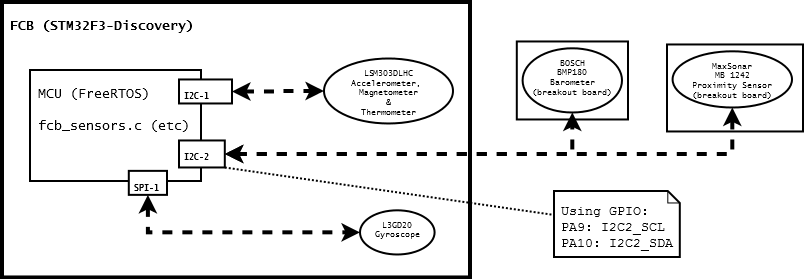
\includegraphics[width=\textwidth]{images/FcbSensorHWConfiguration.png}
    \caption{Sensor overview}
    \label{fig:sensor_hw_overview}
\end{figure}
Since the sensors have no common clock, they send DRDY interrupts to the \texttt{SENSORS} thread independently, see section {sec:real-time-design} on \pageref{sec:real-time-design}. That means that DRDY interrupts arrive at regular intervals with respect to each sensor, but may arrive in any order. All 3 current sensors have differing data rate frequencies.

	\subsection{Sensor axes orientation}
The sensors are not aligned to the Quadcopter body frame by default, so they had to be adjusted. The adjusted axes are green in Figure \ref{fig:sensor_axes_orientation} on page \pageref{fig:sensor_axes_orientation}.
\begin{figure}
    \centering
    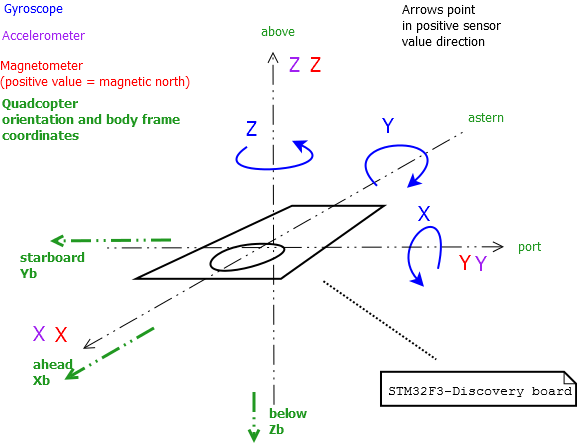
\includegraphics[width=\textwidth]{images/CoordinateFrames.png}
   \caption{Sensor axes orientations}
   \label{fig:sensor_axes_orientation}
\end{figure}

\chapter{Software}

	\section{System Design Overview}
An overview of the entire software architecture can be viewed in Figure \ref{fig:high-level-sw-arch} below. This document mainly concerns the Flight Control Board development.

\begin{figure}[h]
    \centering
    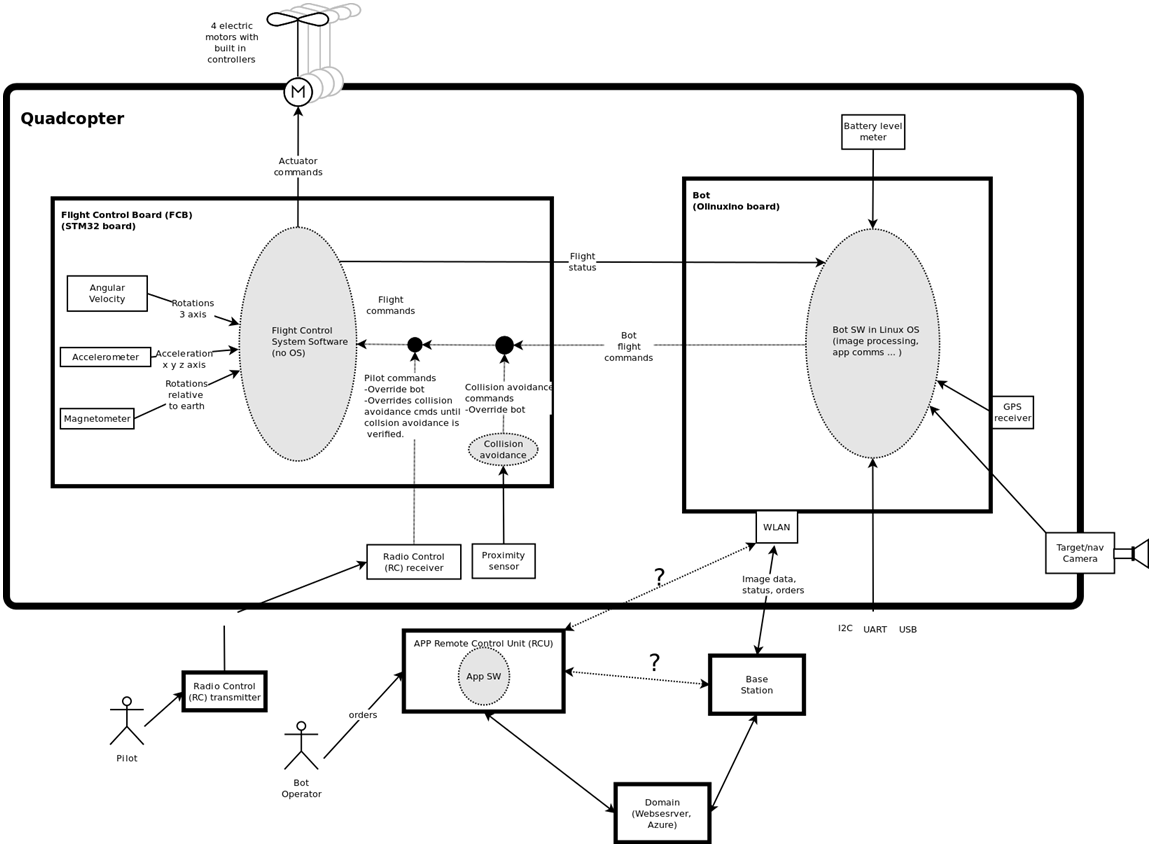
\includegraphics[scale=0.42]{images/high-level-sw-design.png}
    \caption{Overall software architecture}
    \label{fig:high-level-sw-arch}
\end{figure}

As can be viewed in the digram in Figure \ref{fig:fcb-sw-hw-arch}, the Flight Control Board software takes input from a number of sources. Internally, it receives data from the built-in sensors (gyroscope, accelerometer, compass), whereas external commands are received from the Bot SW (Olinuxino board) as well as the radio-controller (RC) receiver. By applying control and output mixing logic (which will be discussed further on), appropriate motor command signals are generated. These are fed to the Electronic speed controllers (ESC), which in turn provide motor actuation. Since the ESCs used on the Dragonfly provide Battery eliminator circuit (BEC) capability, they are able to provide power ($5$ $V$) to the FCB and receiver.

\begin{figure}[h]
    \centering
    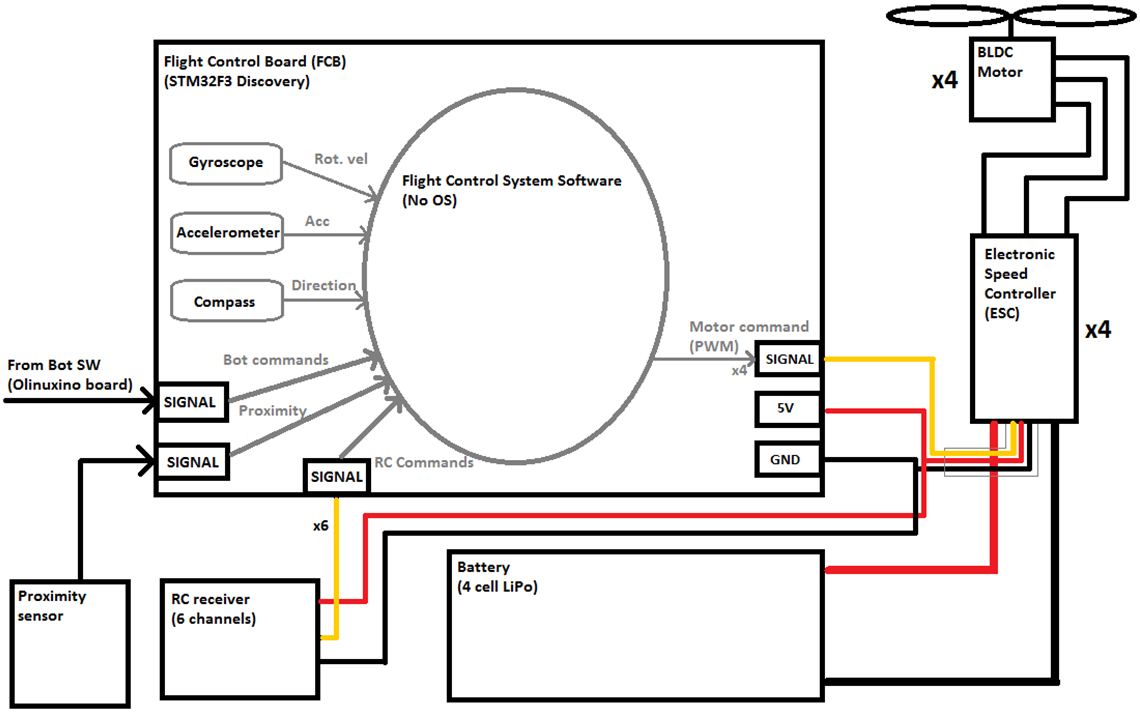
\includegraphics[scale=0.42]{images/fcb-sw-hw-design.png}
    \caption{FCB software architecture and circuit routing overview diagram. Red lines are $5$ $V$, black are ground and yellow are signals.}
    \label{fig:fcb-sw-hw-arch}
\end{figure}

	\section{Real-time Design}
	\label{sec:real-time-design}
Tasks in FreeRTOS have capital names when viewed in the usb COM port console, this convention is retained for this section. The \texttt{SENSORS} task is pended upon the empty \texttt{qFcbSensors} queue, see Figure \ref{fig:freertos-threads-queues-diag} on page \pageref{fig:freertos-threads-queues-diag}.
\begin{figure}[h]
    \centering
    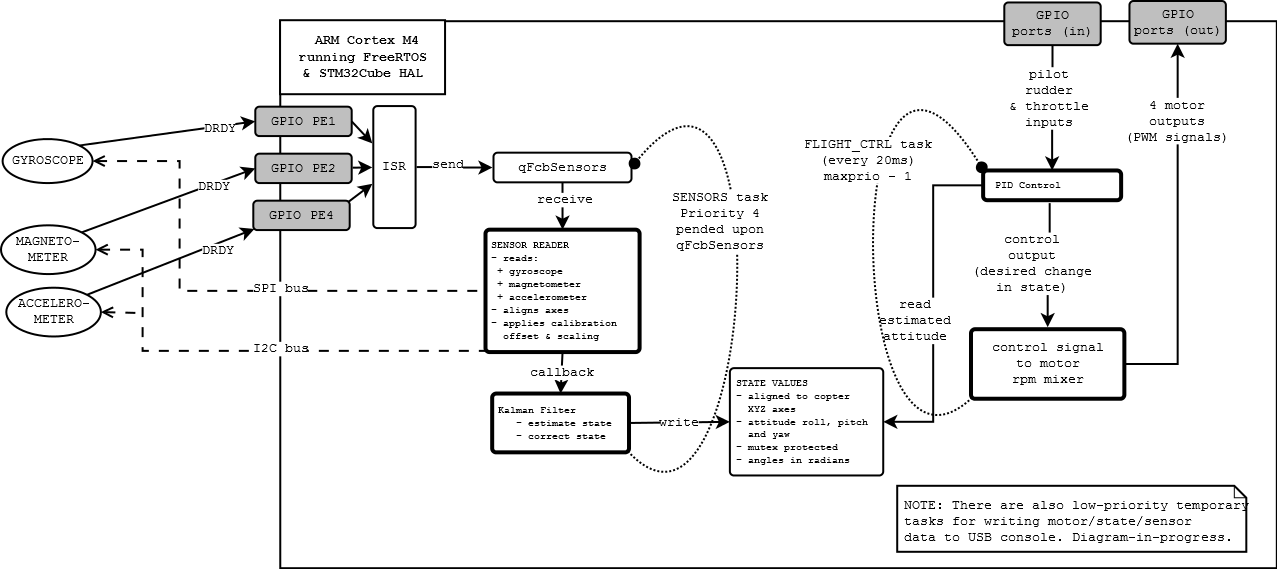
\includegraphics[scale=0.29]{images/FcbThreadsOverview.png}
    \caption{FCB FreeRTOS threads \& queue diagram}
    \label{fig:freertos-threads-queues-diag}
\end{figure}
Whenever one of the sensosr has data ready, an interrupt service routine (ISR) is triggered. The ISR posts a message to the \texttt{qFcbSensors} with the ID of the sensors. The \texttt{SENSORS} task is then released and selects a sensor for reading based on the ID in the queue. Since the sensors have different data rates, the \texttt{SENSORS} task runs at irregular intervals. The task then reads the sensor synchronously and pushes the data to the client, which is the state estimation code. The state estimation code then runs in the \texttt{SENSORS} task context and calculates estimated states.

The \texttt{FLIGHT\_CTRL} task runs in a timed loop every 20 ms. It reads the state estimates and the pilot inputs, runs the PID control code and converts the control signal to motor power signals via the mixer, then starts over.

There are two tasks which do USB communication, one handles reading and the other writing. From the console an operator may request that samples of for instance estimated states or sensor values be printed for analysis for a operator-specified duration. This sampling is done in a temporary tasks that is deleted when either stopped by the operator or until duration has expired.

	\section{Code Documentation}

		\subsection{CMSIS}

		\subsection{STM32F3xx HAL Drivers}
STMicroelectronics provides an extensive library simplifying application interaction with the low-level registers of the MCU. These are known as the Hardware Abstraction Layer (HAL) Drivers, which are a part of the STM32Cube software development package. More detailed documentation on the HAL Drivers library can be found in \cite{stm32f3haldrivers}.

		\subsection{STM32 USB Device Drivers}

		\subsection{STM32F3Discovery Board-specific Package}

		\subsection{FreeRTOS}
FreeRTOS is configured with the \texttt{FreeRTOSConfig.h} file.
		\subsection{FreeRTOS Plus CLI}

		\subsection{FCB Control}

		\subsection{FCB Kalman Filter}
The state estimation code measures the variances of the gyroscope which are then used as initial values for the $Q$ matrix in chapter \ref{chap:state-estimation-theory}. The variance of the measured angle outputs from the rotation matrix which are calculated from the accelerometer and magnetometer readings code is also measured and is used to initialise the $R$ matrix  as well as the diagonal values of the $P$ matrix. The mean of the gyroscope measured angular rates are used to initialise $\dot{\theta_{b}}$.

The $\Delta T$ in equation \ref{eq:state-equation-detailed} is not a constant but is calculated as the interval since the previously received DRDY signal. The reasons are:
\begin{enumerate}
\item The sensors are not syncronised but DRDY interrupts from the 3 different sensors, although inidividually periodic, will still arrive at variable intervals.
\item the estimate is a dead-reckoning or prediction of the current value plus the first derivative multiplied by time. The current value was previously estimated or corrected, hence the time period is since the last DRDY from any sensor.
\end{enumerate}
This applies to both $\Delta T$ in Eq \ref{eq:state-equation-detailed} and $\Delta T$ in Eq \ref{eq:error-covariance-prediction-detailed}.
		\subsection{FCB Communication}

		\subsection{FCB Sensors}
The FCB sensors code is implemented in files i the \texttt{fcb-source/sensors} directory. These file call STM32Cube HAL subroutines for configuring and reading sensors. For the gyroscope, accelerometer and magnetometer the subroutines have been modified to suit the needs of Dragonfly. Most of these modified files are in the \texttt{fcb-source/fcb-drivers} directory. The sensors code also estimates the sensor data rate to be used as $\Delta T$ in the state estimation equations in chapter \ref{chap:state-estimation-theory}.
		\subsection{FCB Utilities}

		\subsection{NanoPB Protocol Buffer}
\appendix
\chapter{GNU Free Documentation License}
This is per instructions at bottom of web page \url{http://www.gnu.org/copyleft/fdl.html} a verbatim copy of this: \url{http://www.gnu.org/licenses/fdl-1.3.txt}
\begin{verbatim}:

                GNU Free Documentation License
                 Version 1.3, 3 November 2008


 Copyright (C) 2000, 2001, 2002, 2007, 2008 Free Software Foundation, Inc.
     <http://fsf.org/>
 Everyone is permitted to copy and distribute verbatim copies
 of this license document, but changing it is not allowed.

0. PREAMBLE

The purpose of this License is to make a manual, textbook, or other
functional and useful document "free" in the sense of freedom: to
assure everyone the effective freedom to copy and redistribute it,
with or without modifying it, either commercially or noncommercially.
Secondarily, this License preserves for the author and publisher a way
to get credit for their work, while not being considered responsible
for modifications made by others.

This License is a kind of "copyleft", which means that derivative
works of the document must themselves be free in the same sense.  It
complements the GNU General Public License, which is a copyleft
license designed for free software.

We have designed this License in order to use it for manuals for free
software, because free software needs free documentation: a free
program should come with manuals providing the same freedoms that the
software does.  But this License is not limited to software manuals;
it can be used for any textual work, regardless of subject matter or
whether it is published as a printed book.  We recommend this License
principally for works whose purpose is instruction or reference.


1. APPLICABILITY AND DEFINITIONS

This License applies to any manual or other work, in any medium, that
contains a notice placed by the copyright holder saying it can be
distributed under the terms of this License.  Such a notice grants a
world-wide, royalty-free license, unlimited in duration, to use that
work under the conditions stated herein.  The "Document", below,
refers to any such manual or work.  Any member of the public is a
licensee, and is addressed as "you".  You accept the license if you
copy, modify or distribute the work in a way requiring permission
under copyright law.

A "Modified Version" of the Document means any work containing the
Document or a portion of it, either copied verbatim, or with
modifications and/or translated into another language.

A "Secondary Section" is a named appendix or a front-matter section of
the Document that deals exclusively with the relationship of the
publishers or authors of the Document to the Document's overall
subject (or to related matters) and contains nothing that could fall
directly within that overall subject.  (Thus, if the Document is in
part a textbook of mathematics, a Secondary Section may not explain
any mathematics.)  The relationship could be a matter of historical
connection with the subject or with related matters, or of legal,
commercial, philosophical, ethical or political position regarding
them.

The "Invariant Sections" are certain Secondary Sections whose titles
are designated, as being those of Invariant Sections, in the notice
that says that the Document is released under this License.  If a
section does not fit the above definition of Secondary then it is not
allowed to be designated as Invariant.  The Document may contain zero
Invariant Sections.  If the Document does not identify any Invariant
Sections then there are none.

The "Cover Texts" are certain short passages of text that are listed,
as Front-Cover Texts or Back-Cover Texts, in the notice that says that
the Document is released under this License.  A Front-Cover Text may
be at most 5 words, and a Back-Cover Text may be at most 25 words.

A "Transparent" copy of the Document means a machine-readable copy,
represented in a format whose specification is available to the
general public, that is suitable for revising the document
straightforwardly with generic text editors or (for images composed of
pixels) generic paint programs or (for drawings) some widely available
drawing editor, and that is suitable for input to text formatters or
for automatic translation to a variety of formats suitable for input
to text formatters.  A copy made in an otherwise Transparent file
format whose markup, or absence of markup, has been arranged to thwart
or discourage subsequent modification by readers is not Transparent.
An image format is not Transparent if used for any substantial amount
of text.  A copy that is not "Transparent" is called "Opaque".

Examples of suitable formats for Transparent copies include plain
ASCII without markup, Texinfo input format, LaTeX input format, SGML
or XML using a publicly available DTD, and standard-conforming simple
HTML, PostScript or PDF designed for human modification.  Examples of
transparent image formats include PNG, XCF and JPG.  Opaque formats
include proprietary formats that can be read and edited only by
proprietary word processors, SGML or XML for which the DTD and/or
processing tools are not generally available, and the
machine-generated HTML, PostScript or PDF produced by some word
processors for output purposes only.

The "Title Page" means, for a printed book, the title page itself,
plus such following pages as are needed to hold, legibly, the material
this License requires to appear in the title page.  For works in
formats which do not have any title page as such, "Title Page" means
the text near the most prominent appearance of the work's title,
preceding the beginning of the body of the text.

The "publisher" means any person or entity that distributes copies of
the Document to the public.

A section "Entitled XYZ" means a named subunit of the Document whose
title either is precisely XYZ or contains XYZ in parentheses following
text that translates XYZ in another language.  (Here XYZ stands for a
specific section name mentioned below, such as "Acknowledgements",
"Dedications", "Endorsements", or "History".)  To "Preserve the Title"
of such a section when you modify the Document means that it remains a
section "Entitled XYZ" according to this definition.

The Document may include Warranty Disclaimers next to the notice which
states that this License applies to the Document.  These Warranty
Disclaimers are considered to be included by reference in this
License, but only as regards disclaiming warranties: any other
implication that these Warranty Disclaimers may have is void and has
no effect on the meaning of this License.

2. VERBATIM COPYING

You may copy and distribute the Document in any medium, either
commercially or noncommercially, provided that this License, the
copyright notices, and the license notice saying this License applies
to the Document are reproduced in all copies, and that you add no
other conditions whatsoever to those of this License.  You may not use
technical measures to obstruct or control the reading or further
copying of the copies you make or distribute.  However, you may accept
compensation in exchange for copies.  If you distribute a large enough
number of copies you must also follow the conditions in section 3.

You may also lend copies, under the same conditions stated above, and
you may publicly display copies.


3. COPYING IN QUANTITY

If you publish printed copies (or copies in media that commonly have
printed covers) of the Document, numbering more than 100, and the
Document's license notice requires Cover Texts, you must enclose the
copies in covers that carry, clearly and legibly, all these Cover
Texts: Front-Cover Texts on the front cover, and Back-Cover Texts on
the back cover.  Both covers must also clearly and legibly identify
you as the publisher of these copies.  The front cover must present
the full title with all words of the title equally prominent and
visible.  You may add other material on the covers in addition.
Copying with changes limited to the covers, as long as they preserve
the title of the Document and satisfy these conditions, can be treated
as verbatim copying in other respects.

If the required texts for either cover are too voluminous to fit
legibly, you should put the first ones listed (as many as fit
reasonably) on the actual cover, and continue the rest onto adjacent
pages.

If you publish or distribute Opaque copies of the Document numbering
more than 100, you must either include a machine-readable Transparent
copy along with each Opaque copy, or state in or with each Opaque copy
a computer-network location from which the general network-using
public has access to download using public-standard network protocols
a complete Transparent copy of the Document, free of added material.
If you use the latter option, you must take reasonably prudent steps,
when you begin distribution of Opaque copies in quantity, to ensure
that this Transparent copy will remain thus accessible at the stated
location until at least one year after the last time you distribute an
Opaque copy (directly or through your agents or retailers) of that
edition to the public.

It is requested, but not required, that you contact the authors of the
Document well before redistributing any large number of copies, to
give them a chance to provide you with an updated version of the
Document.


4. MODIFICATIONS

You may copy and distribute a Modified Version of the Document under
the conditions of sections 2 and 3 above, provided that you release
the Modified Version under precisely this License, with the Modified
Version filling the role of the Document, thus licensing distribution
and modification of the Modified Version to whoever possesses a copy
of it.  In addition, you must do these things in the Modified Version:

A. Use in the Title Page (and on the covers, if any) a title distinct
   from that of the Document, and from those of previous versions
   (which should, if there were any, be listed in the History section
   of the Document).  You may use the same title as a previous version
   if the original publisher of that version gives permission.
B. List on the Title Page, as authors, one or more persons or entities
   responsible for authorship of the modifications in the Modified
   Version, together with at least five of the principal authors of the
   Document (all of its principal authors, if it has fewer than five),
   unless they release you from this requirement.
C. State on the Title page the name of the publisher of the
   Modified Version, as the publisher.
D. Preserve all the copyright notices of the Document.
E. Add an appropriate copyright notice for your modifications
   adjacent to the other copyright notices.
F. Include, immediately after the copyright notices, a license notice
   giving the public permission to use the Modified Version under the
   terms of this License, in the form shown in the Addendum below.
G. Preserve in that license notice the full lists of Invariant Sections
   and required Cover Texts given in the Document's license notice.
H. Include an unaltered copy of this License.
I. Preserve the section Entitled "History", Preserve its Title, and add
   to it an item stating at least the title, year, new authors, and
   publisher of the Modified Version as given on the Title Page.  If
   there is no section Entitled "History" in the Document, create one
   stating the title, year, authors, and publisher of the Document as
   given on its Title Page, then add an item describing the Modified
   Version as stated in the previous sentence.
J. Preserve the network location, if any, given in the Document for
   public access to a Transparent copy of the Document, and likewise
   the network locations given in the Document for previous versions
   it was based on.  These may be placed in the "History" section.
   You may omit a network location for a work that was published at
   least four years before the Document itself, or if the original
   publisher of the version it refers to gives permission.
K. For any section Entitled "Acknowledgements" or "Dedications",
   Preserve the Title of the section, and preserve in the section all
   the substance and tone of each of the contributor acknowledgements
   and/or dedications given therein.
L. Preserve all the Invariant Sections of the Document,
   unaltered in their text and in their titles.  Section numbers
   or the equivalent are not considered part of the section titles.
M. Delete any section Entitled "Endorsements".  Such a section
   may not be included in the Modified Version.
N. Do not retitle any existing section to be Entitled "Endorsements"
   or to conflict in title with any Invariant Section.
O. Preserve any Warranty Disclaimers.

If the Modified Version includes new front-matter sections or
appendices that qualify as Secondary Sections and contain no material
copied from the Document, you may at your option designate some or all
of these sections as invariant.  To do this, add their titles to the
list of Invariant Sections in the Modified Version's license notice.
These titles must be distinct from any other section titles.

You may add a section Entitled "Endorsements", provided it contains
nothing but endorsements of your Modified Version by various
parties--for example, statements of peer review or that the text has
been approved by an organization as the authoritative definition of a
standard.

You may add a passage of up to five words as a Front-Cover Text, and a
passage of up to 25 words as a Back-Cover Text, to the end of the list
of Cover Texts in the Modified Version.  Only one passage of
Front-Cover Text and one of Back-Cover Text may be added by (or
through arrangements made by) any one entity.  If the Document already
includes a cover text for the same cover, previously added by you or
by arrangement made by the same entity you are acting on behalf of,
you may not add another; but you may replace the old one, on explicit
permission from the previous publisher that added the old one.

The author(s) and publisher(s) of the Document do not by this License
give permission to use their names for publicity for or to assert or
imply endorsement of any Modified Version.


5. COMBINING DOCUMENTS

You may combine the Document with other documents released under this
License, under the terms defined in section 4 above for modified
versions, provided that you include in the combination all of the
Invariant Sections of all of the original documents, unmodified, and
list them all as Invariant Sections of your combined work in its
license notice, and that you preserve all their Warranty Disclaimers.

The combined work need only contain one copy of this License, and
multiple identical Invariant Sections may be replaced with a single
copy.  If there are multiple Invariant Sections with the same name but
different contents, make the title of each such section unique by
adding at the end of it, in parentheses, the name of the original
author or publisher of that section if known, or else a unique number.
Make the same adjustment to the section titles in the list of
Invariant Sections in the license notice of the combined work.

In the combination, you must combine any sections Entitled "History"
in the various original documents, forming one section Entitled
"History"; likewise combine any sections Entitled "Acknowledgements",
and any sections Entitled "Dedications".  You must delete all sections
Entitled "Endorsements".


6. COLLECTIONS OF DOCUMENTS

You may make a collection consisting of the Document and other
documents released under this License, and replace the individual
copies of this License in the various documents with a single copy
that is included in the collection, provided that you follow the rules
of this License for verbatim copying of each of the documents in all
other respects.

You may extract a single document from such a collection, and
distribute it individually under this License, provided you insert a
copy of this License into the extracted document, and follow this
License in all other respects regarding verbatim copying of that
document.


7. AGGREGATION WITH INDEPENDENT WORKS

A compilation of the Document or its derivatives with other separate
and independent documents or works, in or on a volume of a storage or
distribution medium, is called an "aggregate" if the copyright
resulting from the compilation is not used to limit the legal rights
of the compilation's users beyond what the individual works permit.
When the Document is included in an aggregate, this License does not
apply to the other works in the aggregate which are not themselves
derivative works of the Document.

If the Cover Text requirement of section 3 is applicable to these
copies of the Document, then if the Document is less than one half of
the entire aggregate, the Document's Cover Texts may be placed on
covers that bracket the Document within the aggregate, or the
electronic equivalent of covers if the Document is in electronic form.
Otherwise they must appear on printed covers that bracket the whole
aggregate.


8. TRANSLATION

Translation is considered a kind of modification, so you may
distribute translations of the Document under the terms of section 4.
Replacing Invariant Sections with translations requires special
permission from their copyright holders, but you may include
translations of some or all Invariant Sections in addition to the
original versions of these Invariant Sections.  You may include a
translation of this License, and all the license notices in the
Document, and any Warranty Disclaimers, provided that you also include
the original English version of this License and the original versions
of those notices and disclaimers.  In case of a disagreement between
the translation and the original version of this License or a notice
or disclaimer, the original version will prevail.

If a section in the Document is Entitled "Acknowledgements",
"Dedications", or "History", the requirement (section 4) to Preserve
its Title (section 1) will typically require changing the actual
title.


9. TERMINATION

You may not copy, modify, sublicense, or distribute the Document
except as expressly provided under this License.  Any attempt
otherwise to copy, modify, sublicense, or distribute it is void, and
will automatically terminate your rights under this License.

However, if you cease all violation of this License, then your license
from a particular copyright holder is reinstated (a) provisionally,
unless and until the copyright holder explicitly and finally
terminates your license, and (b) permanently, if the copyright holder
fails to notify you of the violation by some reasonable means prior to
60 days after the cessation.

Moreover, your license from a particular copyright holder is
reinstated permanently if the copyright holder notifies you of the
violation by some reasonable means, this is the first time you have
received notice of violation of this License (for any work) from that
copyright holder, and you cure the violation prior to 30 days after
your receipt of the notice.

Termination of your rights under this section does not terminate the
licenses of parties who have received copies or rights from you under
this License.  If your rights have been terminated and not permanently
reinstated, receipt of a copy of some or all of the same material does
not give you any rights to use it.


10. FUTURE REVISIONS OF THIS LICENSE

The Free Software Foundation may publish new, revised versions of the
GNU Free Documentation License from time to time.  Such new versions
will be similar in spirit to the present version, but may differ in
detail to address new problems or concerns.  See
http://www.gnu.org/copyleft/.

Each version of the License is given a distinguishing version number.
If the Document specifies that a particular numbered version of this
License "or any later version" applies to it, you have the option of
following the terms and conditions either of that specified version or
of any later version that has been published (not as a draft) by the
Free Software Foundation.  If the Document does not specify a version
number of this License, you may choose any version ever published (not
as a draft) by the Free Software Foundation.  If the Document
specifies that a proxy can decide which future versions of this
License can be used, that proxy's public statement of acceptance of a
version permanently authorizes you to choose that version for the
Document.

11. RELICENSING

"Massive Multiauthor Collaboration Site" (or "MMC Site") means any
World Wide Web server that publishes copyrightable works and also
provides prominent facilities for anybody to edit those works.  A
public wiki that anybody can edit is an example of such a server.  A
"Massive Multiauthor Collaboration" (or "MMC") contained in the site
means any set of copyrightable works thus published on the MMC site.

"CC-BY-SA" means the Creative Commons Attribution-Share Alike 3.0
license published by Creative Commons Corporation, a not-for-profit
corporation with a principal place of business in San Francisco,
California, as well as future copyleft versions of that license
published by that same organization.

"Incorporate" means to publish or republish a Document, in whole or in
part, as part of another Document.

An MMC is "eligible for relicensing" if it is licensed under this
License, and if all works that were first published under this License
somewhere other than this MMC, and subsequently incorporated in whole or
in part into the MMC, (1) had no cover texts or invariant sections, and
(2) were thus incorporated prior to November 1, 2008.

The operator of an MMC Site may republish an MMC contained in the site
under CC-BY-SA on the same site at any time before August 1, 2009,
provided the MMC is eligible for relicensing.


ADDENDUM: How to use this License for your documents

To use this License in a document you have written, include a copy of
the License in the document and put the following copyright and
license notices just after the title page:

    Copyright (c)  YEAR  YOUR NAME.
    Permission is granted to copy, distribute and/or modify this document
    under the terms of the GNU Free Documentation License, Version 1.3
    or any later version published by the Free Software Foundation;
    with no Invariant Sections, no Front-Cover Texts, and no Back-Cover Texts.
    A copy of the license is included in the section entitled "GNU
    Free Documentation License".

If you have Invariant Sections, Front-Cover Texts and Back-Cover Texts,
replace the "with...Texts." line with this:

    with the Invariant Sections being LIST THEIR TITLES, with the
    Front-Cover Texts being LIST, and with the Back-Cover Texts being LIST.

If you have Invariant Sections without Cover Texts, or some other
combination of the three, merge those two alternatives to suit the
situation.

If your document contains nontrivial examples of program code, we
recommend releasing these examples in parallel under your choice of
free software license, such as the GNU General Public License,
to permit their use in free software.

\end{verbatim}
\begin{thebibliography}{99}
\bibitem{stenberg} Model-based Design Development and Control of a Wind Resistant Multirotor UAV, C. Månsson, D. Stenberg, Dept. of Automatic Control LTH 2014, \url{http://www.control.lth.se/Publication/5947.html}
\bibitem{bresciani} Modelling, Identification and Control of a Quadrotor Helicopter, T. Bresciani, Dept. of Automatic Control LTH 2008, http://\url{www.control.lth.se/Publication/5823.html}
\bibitem{stm32f3discovery1} UM1562 User Manual: Getting started with software and firmware environments for the STM32F3DISCOVERY Kit, ST Microelectronics, \url{http://www.st.com/web/catalog/tools/FM116/SC959/SS1532/PF254044}
\bibitem{stm32f303refman} RM0316 User Manual: Reference Manual for  STM32F303xB/C, STM32F303x6/8, STM32F328x8 and STM32F358xC advanced ARM®-based 32-bit MCUs, ST Microelectronics, \url{http://www.st.com/web/en/resource/technical/document/reference_manual/DM00043574.pdf}
\bibitem{stm32f3discovery2}UM1570 User Manual: STM32F3DISCOVERY Discovery kit for STM32F303xx microcontrollers, ST Microelectronics, http://\url{www.st.com/web/catalog/tools/FM116/SC959/SS1532/PF254044}
\bibitem{stm32f3progman}PM0214 Programming Manual: STM32F3 and STM32F4 Series Cortex®-M4 programming manual, ST Microelectronics, http://\url{www.st.com/st-web-ui/static/active/en/resource/technical/document/programming_manual/DM00046982.pdf}
\bibitem{stm32f3haldrivers}UM1786 User Manual: Description of STM32F3xx HAL drivers, ST Microelectronics, http://\url{http://www.st.com/st-web-ui/static/active/en/resource/technical/document/user_manual/DM00122016.pdf}
\bibitem{spektrumar610userguide}Spektrum AR610 User Guide, Spektrum 2012, \url{https://www.spektrumrc.com/ProdInfo/Files/SPMAR610_Manual_EN.pdf}
\end{thebibliography}

\end{document}                  % End of document
